\chapter{Мультисекущий Бройден с адаптивным окном}\label{ch:sp-broyden-theory}
%% ============================================================

В этой главе анализируется мультисекущее обновление Бройдена с
адаптивным выбором глубины окна~--- квазиньютоновский метод решения
системы $F(x)=0$, в котором новая аппроксимация якобиана $B_{k+1}$
удовлетворяет $p+1$ секущим условиям из текущего окна последних шагов
вместо одного, как в классическом Бройдене. Замкнутая матричная
форма мультисекущего обновления для несимметричного бройденовского
семейства приведена Шнабелем~\cite{schnabel1983}; здесь она снабжается
адаптивным правилом выбора глубины $p$ и подвергается локальному
анализу в форме теоремы об ограниченном ухудшении (bounded
deterioration). Исторический предшественник~--- Projected Broyden Гэя и
Шнабеля~\cite{gay_schnabel1978}, ранг-1 специализация мультисекущего
обновления при сохранении инварианта $B_k s_j = y_j$ ($j<k$)~---
обсуждается в~\S\ref{sec:highdim} в связи с limited-memory реализацией.

Основные результаты главы:
теорема~\ref{thm:bd}~--- точное разложение и оценка bounded
deterioration по фробениусовой норме ошибки $E_k = B_k - \Jstar$
с явной геометрической константой $C_{\mathrm{PB}} = L(1+C_s/2)\sqrt{p+1}\,\kappa_p$,
где $\kappa_p = \kappa(S_p)$ контролируется адаптивным порогом
$\mathrm{cond}(G_p)<\tau$;
следствие~\ref{cor:subspace-alignment}~--- безусловная
$O(\rho_k)$-аппроксимация якобиана на подпространстве прошлых шагов
$\mathrm{col}\,S_p$ (структурное преимущество над классическим
Бройденом). Численные эксперименты (\S\ref{sec:spb_numerics}) и
limited-memory вариант L-PB (\S\ref{sec:highdim}) дополняют
теоретическую часть.

\noindent\textbf{Обозначения и предположения главы.}\enskip
Рассматривается задача поиска корня $F(x) = 0$ с
непрерывно-дифференцируемым отображением $F\colon\RR^n \to \RR^n$
и якобианом $J(x) = F'(x)$. Обозначим $x^*$~--- корень системы
($F(x^*) = 0$), $\Jstar = J(x^*)$, $s_k = x_{k+1} - x_k$,
$y_k = F(x_{k+1}) - F(x_k)$, $E_k = B_k - \Jstar$~--- ошибку
аппроксимации якобиана. Во всех теоретических утверждениях
главы~2 предполагается, что якобиан липшицев на некоторой открытой
окрестности $\mathcal{O} \subset \RR^n$ точки $x^*$:
\begin{equation}\label{eq:lipschitz}
  \Norm{J(x) - J(y)} \le L\,\Norm{x - y},
  \qquad x, y \in \mathcal{O}.
\end{equation}
Это стандартное предположение для анализа локальной сходимости
квазиньютоновских методов; см.~\cite{dennis1977,dennis1996}.

\medskip

Идея мультисекущего обновления: вместо одного секущего условия
$B_{k+1} s_k = y_k$, удовлетворяемого классическим Бройденом, потребуем,
чтобы $B_{k+1}$ согласовывалось со \emph{всеми} парами $(s_j, y_j)$ из
текущего окна $j = k{-}p, \ldots, k$, то~есть
$B_{k+1}\,S_p = Y_p$. Среди всех матриц с этим свойством выбирается
ближайшая к $B_k$ по фробениусовой норме~--- это и~есть мультисекущая
форма Шнабеля~\cite{schnabel1983}, замкнутый вид которой приведён
ниже.

\begin{definition}[Мультисекущее обновление Бройдена]\label{def:sp_update}
Пусть задана глубина окна $p \geq 0$ и пусть шаги
$s_k, s_{k-1}, \ldots, s_{k-p}$ линейно независимы; обозначим
\[
  S_p = [s_k \mid s_{k-1} \mid \cdots \mid s_{k-p}] \in \RR^{n\times(p+1)},
  \qquad
  Y_p = [y_k \mid y_{k-1} \mid \cdots \mid y_{k-p}],
  \qquad
  G_p = S_p^\top S_p.
\]
\emph{Мультисекущее обновление} (MS-обновление) задаётся формулой
\begin{equation}\label{eq:sp_update}
  B_{k+1} = B_k + (Y_p - B_k\,S_p)\,G_p^{-1}\,S_p^\top.
\end{equation}
\end{definition}

\begin{remark}[Соглашение об обозначениях]\label{rem:notation}
Параметр $p$ обозначает число \emph{прошлых} секущих, входящих в окно
наряду с текущей; всего окно содержит $p+1$ пару. Текущий шаг $s_k$
стоит \emph{первым} столбцом матрицы $S_p$. В отличие от этого,
в общей формуле~\eqref{eq:general} столбцы $S_m$ расположены в
хронологическом порядке: от старых к новым.
\end{remark}

\begin{remark}[Минимум-Фробениус характеризация]\label{rem:ms_minfrob}
Формула~\eqref{eq:sp_update} есть единственная матрица $B_{k+1}$,
удовлетворяющая $B_{k+1}\,S_p = Y_p$ и минимизирующая $\|B_{k+1} - B_k\|_F$;
ранг обновления $B_{k+1} - B_k = (Y_p - B_k S_p) G_p^{-1} S_p^\top$ не
превосходит $p+1$. Это~--- классическая характеризация мультисекущей
формы для несимметричного бройденовского семейства~\cite[ур.~(2.5)]{schnabel1983};
ср.~также унифицированную классификацию Type-I/Type-II у Фана и
Саада~\cite[ур.~(26)]{fang2009}, где Type-II вариант оказывается
эквивалентным ускорению Андерсона.
При $p=0$ матрица $G_0 = \|s_k\|^2$ и формула~\eqref{eq:sp_update}
переходит в классическое обновление Бройдена~\eqref{eq:good_broyden}.
\end{remark}

\begin{remark}[Численная форма]\label{rem:ms_numerical}
Прямое обращение $G_p$ нежелательно при плохой обусловленности.
Поскольку $G_p \succ 0$, на практике используются:
\textbf{(i)} разложение Холецкого $G_p = LL^\top$ с двумя треугольными
подстановками для решения $G_p X = S_p^\top$ (стоимость $O(p^3)$);
\textbf{(ii)} тонкое QR-разложение $S_p = QR$, дающее
$G_p^{-1} S_p^\top = R^{-1} Q^\top$ и более устойчивое при умеренно
плохой обусловленности~\cite[\S 5.3.3]{golub2013}. Адаптивный отбор
глубины в Алгоритме~\ref{alg:sp_broyden} (условие
$\mathrm{cond}(G_p)<\tau$) удерживает $\kappa_p = \kappa(S_p) \le \sqrt{\tau}$,
что и~обосновывает выбор порога~$\tau$ через входящий в~оценку
теоремы~\ref{thm:bd} множитель $\sqrt{p+1}\,\kappa_p$ в~$C_{\mathrm{PB}}$
(см.\ замечание~\ref{rem:csp-meaning}).
\end{remark}

\begin{remark}[Историческая привязка]\label{rem:ms_history}
Мультисекущее обновление в форме~\eqref{eq:sp_update} выписано Шнабелем
в техотчёте~1983~\cite{schnabel1983} как часть унифицированного
рассмотрения мультисекущих расширений сразу для четырёх семейств
(Бройден, PSB, DFP, BFGS). Исторически ранее Гэй и
Шнабель~\cite{gay_schnabel1978} рассматривали ранг-1 \emph{Projected
Broyden} (Algorithm~II), сохраняющий прошлые секущие напрямую через
проектирование направления $v_k$ на ортогональное дополнение к
$\mathrm{span}(s_{k-1},\ldots,s_{k-p})$; их Theorem~2.1 показывает, что
эта ранг-1 конструкция совпадает с~\eqref{eq:sp_update} при выполнении
индуктивного инварианта $B_k s_j = y_j$ ($j<k$) и~даёт минимум-Фробениус
обновление в~указанном классе. В~настоящей работе формулировка~\eqref{eq:sp_update}
выбрана за~основу как чисто алгебраическая (не~требует индуктивного
инварианта), а~ранг-1 специализация возвращается в~\S\ref{sec:highdim}
ради limited-memory реализации через формулу
Шермана--Моррисона. Установленные у~Гэя и~Шнабеля свойства~--- bounded
deterioration (Th.~4.2) и~локальная Q-сверхлинейная сходимость
(Th.~4.5)~--- в~настоящей главе уточняются: теорема~\ref{thm:bd} даёт
точное разложение Фробениус-нормы~ошибки и~явную геометрическую
константу, а~следствие~\ref{cor:subspace-alignment}~--- безусловный
$O(\rho_k)$-контроль ошибки на~всём подпространстве $\mathrm{col}\,S_p$
(в~\cite{gay_schnabel1978} в~явном виде эти факты не~приводятся).
\end{remark}

\medskip

Полный алгоритм приведён в Алгоритме~\ref{alg:sp_broyden}.

\begin{breakablealgorithm}
\caption{Мультисекущий Бройден с адаптивным окном
         $(F,\,x_0,\,p_{\max},\,\widetilde{B},\,\tau,\,\varepsilon,\,\mathtt{accumulate})$}
\label{alg:sp_broyden}
\begin{algorithmic}
\Require $F\colon \mathbb{R}^n \to \mathbb{R}^n$,\ $x_0 \in \mathbb{R}^n$,\
         $p_{\max} \geq 0$,\
         $\widetilde{B} \in \mathbb{R}^{n \times n}$
         \Comment{опорная матрица алгоритма, куда
                  происходит сброс в режиме пересборки; обычно $I_n$.
                  Не путать с базовой матрицей $\widehat{B}_k$ в формуле обновления.},\
         $\tau > 0$,\ $\varepsilon > 0$,\
         $\mathtt{accumulate} \in \{\text{true},\text{false}\}$
\State $B_0 \leftarrow \widetilde{B}$,\quad $k \leftarrow 0$
\While{$\|F(x_k)\| \geq \varepsilon$}
  \State Решить $B_k\,d_k = -F(x_k)$
  \State $x_{k+1} \leftarrow x_k + d_k$
  \State $s_k \leftarrow d_k$,\quad $y_k \leftarrow F(x_{k+1}) - F(x_k)$
  %------------------------------------------------------------
  \State \textbf{Адаптивный выбор глубины окна:}
  \State $p \leftarrow 0$
  \For{$p' = 1,\ldots,\min(p_{\max},\,k)$}
    \State $S_{p'} \leftarrow [s_k \mid s_{k-1} \mid \cdots \mid s_{k-p'}]$
      \hfill\Comment{$n\times(p'{+}1)$ матрица}
    \If{$\operatorname{cond}(S_{p'}^\top S_{p'}) < \tau$}
      \State $p \leftarrow p'$
    \Else
      \State \textbf{break}
    \EndIf
  \EndFor
  %------------------------------------------------------------
  \State \textbf{MS-обновление якобиана:}
  \If{$\mathtt{accumulate}$}
    \State $\widehat{B}_k \leftarrow B_k$
  \Else
    \State $\widehat{B}_k \leftarrow \widetilde{B}$
  \EndIf
  \State $S_p \leftarrow [s_k \mid s_{k-1} \mid \cdots \mid s_{k-p}]$,\quad
         $Y_p \leftarrow [y_k \mid y_{k-1} \mid \cdots \mid y_{k-p}]$
  \State $G_p \leftarrow S_p^\top S_p$
       \hfill\Comment{$(p{+}1)\times(p{+}1)$, симметричный, $\succ 0$}
  \State $B_{k+1} \leftarrow \widehat{B}_k +
    (Y_p - \widehat{B}_k S_p)\,G_p^{-1}\,S_p^\top$
       \hfill\Comment{ранг $\le p{+}1$; при $p{=}0$~--- классический Бройден}
  \State $k \leftarrow k + 1$
\EndWhile
\Return $x_k$
\end{algorithmic}
\end{breakablealgorithm}

\begin{remark}[Связь с таксономией обновлений]\label{rem:taxonomy}
Опция $\mathtt{accumulate}$ переключает между двумя строками
классификации Fang--Saad~\cite{fang2009} для мультисекущих
бройденовских обновлений. При $\mathtt{accumulate}=\text{true}$
(базовый режим всех экспериментов главы) в качестве опорной матрицы
$\widehat B_k$ берётся текущее $B_k$, накопившее историю прошлых
обновлений; при $\mathtt{accumulate}=\text{false}$~--- фиксированное
$\widetilde B$ (типично~$I$), и обновление становится Type-II
вариантом, эквивалентным ускорению Андерсона~\cite{anderson1965}
(см.\ ур.~(26) в~\cite{fang2009}). В обоих случаях формула
обновления одна и~та~же~--- ранг-$(p{+}1)$ мультисекущая.
\end{remark}

\begin{remark}[Сложность]\label{rem:complexity}
Доминирующие операции на итерацию: формирование $\widehat B_k S_p$
(плотное матрично-матричное произведение, $O(n^2 p)$); решение
$(p{+}1)\times(p{+}1)$-системы $G_p X = S_p^\top$ через разложение
Холецкого ($O(p^3)$); решение $B_k d_k = -F(x_k)$ через LU
($O(n^3)$). При $p\ll n$ доминирует LU.
Limited-memory вариант~\S\ref{sec:highdim} убирает $O(n^2)$-память
и $O(n^3)$-стоимость LU за счёт специализации к ранг-1 случаю
с~Шерманом--Моррисоном.
\end{remark}

%% ============================================================
\section{Качество аппроксимации якобиана}\label{sec:sp-broyden-proof}
%% ============================================================

%% ============================================================
%% Bounded deterioration для мультисекущего Бройдена
%% ============================================================

%% --- Локальная оценка длины шага ---

\begin{lemma}[Локальная оценка длины шага через расстояние до корня]
\label{lem:step-bound}
Пусть якобиан $J$ удовлетворяет условию Липшица~\eqref{eq:lipschitz}
с константой $L$ на шаре $B(x^{*}, \delta_0) := \{x : \|x - x^{*}\| \le \delta_0\}$,
$F(x^{*}) = 0$, и пусть $B_j$ обратима с $\|B_j^{-1}\| \le M$
для всех $j \in \{k{-}p,\ldots,k\}$. Тогда для каждого
$j \in \{k{-}p,\ldots,k\}$ с $x_j \in B(x^{*}, \delta_0)$ длина шага
$s_j = -B_j^{-1} F(x_j)$ удовлетворяет
\begin{equation}\label{eq:step-bound-Cs}
  \|s_j\| \;\le\; C_s\,\|x_j - x^{*}\|,
  \qquad
  C_s \;:=\; M\Big(\|\Jstar\| + \tfrac{L}{2}\,\delta_0\Big),
\end{equation}
где $\|\Jstar\|$~--- спектральная (операторная) норма $J(x^{*})$.
\end{lemma}

\begin{proof}
По интегральной формуле Ньютона--Лейбница и $F(x^{*}) = 0$:
\[
  F(x_j) \;=\; F(x_j) - F(x^{*})
  \;=\; \left(\int_{0}^{1} J\!\big(x^{*} + t(x_j - x^{*})\big)\,dt\right)(x_j - x^{*}).
\]
Применяя оценку Липшица $\|J(x^{*} + \tau(x_j-x^{*})) - \Jstar\| \le L\,\tau\,\|x_j-x^{*}\|$
и интегрируя:
\[
  \left\|\int_{0}^{1} J\!\big(x^{*} + t(x_j-x^{*})\big)\,dt\right\|
  \;\le\; \|\Jstar\| + \tfrac{L}{2}\,\|x_j - x^{*}\|
  \;\le\; \|\Jstar\| + \tfrac{L}{2}\,\delta_0.
\]
Отсюда $\|F(x_j)\| \le (\|\Jstar\| + \tfrac{L}{2}\,\delta_0)\,\|x_j - x^{*}\|$.
По условию леммы $\|s_j\| \le M\,\|F(x_j)\|$, что даёт~\eqref{eq:step-bound-Cs}.
\end{proof}

\begin{remark}[Локальная фаза и пребывание траектории в шаре]
\label{rem:trajectory-confinement}
Лемма~\ref{lem:step-bound} требует $x_j \in B(x^*,\delta_0)$ для всех
$j$ из рассматриваемого окна. Индуктивное обоснование пребывания
траектории в~шаре~--- стандартный шаг локальной теории
квазиньютоновских методов (Dennis--Schnabel,
\cite[Th.~8.2.1]{dennis1996}; ср.~также~\cite[\S 6.4]{bfgs}): при
достаточно близком старте~$x_0$ и достаточно малом~$\|E_0\|$ оценка
теоремы~\ref{thm:bd} ниже гарантирует, что $\{x_k\}$ не покидает
$B(x^*,\delta_0)$. В~настоящей работе анализ ограничен этой локальной
фазой; для всего последующего анализа пребывание окна
$x_{k-p},\ldots,x_k\in B(x^*,\delta_0)$ принимается как стандартное
допущение локального анализа.
\end{remark}

%% --- Основная теорема ---

\begin{theorem}[Bounded deterioration для мультисекущего Бройдена]\label{thm:bd}
Пусть $S_p\in\RR^{n\times(p+1)}$ имеет полный столбцовый ранг,
$Y_p$ и $G_p = S_p^\top S_p$ определены как в опр.~\ref{def:sp_update},
а $B_{k+1}$ задано MS-обновлением~\eqref{eq:sp_update}. Пусть якобиан
$J(x)$ удовлетворяет условию Липшица~\eqref{eq:lipschitz} с константой
$L$ на открытой окрестности $\mathcal{O}\subset\RR^n$, содержащей
$x^{*}$, все точки $x_j$ и отрезки $\{x_j+t s_j : t\in[0,1]\}$ для
$j=k-p,\ldots,k$. Обозначим $\Jstar = J(x^*)$, $E_k = B_k - \Jstar$,
\[
  \Pi_k = S_p\,G_p^{-1}\,S_p^\top \quad\text{(ортогональный проектор на
  $\mathrm{col}\,S_p$)},
  \qquad
  \Pi_k^\perp = I - \Pi_k.
\]

Тогда:

\begin{enumerate}
\item[\textup{(a)}] \textbf{Точное разложение.}
\begin{equation}\label{eq:exact_decomp}
  \|E_{k+1}\|_F^2
  = \|E_k\|_F^2 - \|E_k\,\Pi_k\|_F^2 + \Delta_k,
\end{equation}
где
\begin{equation}\label{eq:Delta_def}
  \Delta_k = \operatorname{tr}\!\bigl(G_p^{-1}\,(Y_p - \Jstar\!S_p)^\top
  (Y_p - \Jstar\!S_p)\bigr).
\end{equation}

\item[\textup{(b)}] \textbf{Bounded deterioration.}
Пусть выполнены условия леммы~\ref{lem:step-bound} с константой $C_s$
(в~частности, $B(x^{*},\delta_0)\subset\mathcal{O}$, так что
$\|s_j\|\le C_s\|x_j-x^{*}\|$ для $j=k-p,\ldots,k$).
Обозначим
\begin{equation}\label{eq:rho-window}
  \rho_k \;:=\; \max_{k-p\,\le\,j\,\le\,k}\,\|x_j - x^{*}\|,
  \qquad
  \kappa_p \;:=\; \kappa(S_p)
  = \frac{\sigma_{\max}(S_p)}{\sigma_{\min}(S_p)}.
\end{equation}
Тогда
\begin{equation}\label{eq:bd_squared}
  \|E_{k+1}\|_F^2 \;\le\; \|E_k\|_F^2 \;-\; \|E_k\,\Pi_k\|_F^2
  \;+\; C_{\mathrm{PB}}^2\,\rho_k^2,
  \qquad
  C_{\mathrm{PB}} := L\,(1 + C_s/2)\,\sqrt{p+1}\,\kappa_p.
\end{equation}
\end{enumerate}
\end{theorem}

\begin{remark}[Расшифровка $C_{\mathrm{PB}}$]\label{rem:csp-meaning}
Структура константы $C_{\mathrm{PB}}$ прозрачна: $L$~--- константа Липшица
якобиана; $C_s$~--- типичный размер шага относительно расстояния до
корня (лемма~\ref{lem:step-bound}); $\sqrt{p+1}$~--- цена расширения окна
секущих; $\kappa_p$~--- обусловленность окна $S_p$. Адаптивный порог
$\mathrm{cond}(G_p)<\tau$ Алгоритма~\ref{alg:sp_broyden} обеспечивает
$\kappa_p\le\sqrt{\tau}$, так что $C_{\mathrm{PB}}\le L(1+C_s/2)\sqrt{\tau(p+1)}$.
В классической форме Бройдена ($p=0$, $\Pi_k = s_k s_k^\top/\|s_k\|^2$,
$\kappa_0 = 1$) эта оценка переходит в стандартную bounded deterioration
с $C_{\mathrm{Br}} = L(1+C_s/2)$,~ср.~\cite{broyden1973,dennis1996}.
Константа $M = \sup_j\|B_j^{-1}\|$ из леммы~\ref{lem:step-bound},
входящая в $C_s$, конечна при $\|E_j\|<\sigma_{\min}(\Jstar)$ (неравенство
Вейля).
\end{remark}

\begin{proof}

\textbf{Шаг~1: разложение $E_{k+1}$.}
Подставим определение MS-обновления~\eqref{eq:sp_update}:
\begin{align}
  E_{k+1}
  &= B_k - \Jstar + (Y_p - B_k S_p)\,G_p^{-1}\,S_p^\top \notag\\
  &= E_k + \bigl[(Y_p - \Jstar\!S_p) - E_k\,S_p\bigr]\,G_p^{-1}\,S_p^\top \notag\\
  &= E_k\,(I - S_p\,G_p^{-1}\,S_p^\top)
     + (Y_p - \Jstar\!S_p)\,G_p^{-1}\,S_p^\top. \label{eq:Ek1_full}
\end{align}
То есть:
\begin{equation}\label{eq:Ek1_compact}
  E_{k+1} = E_k\,\Pi_k^\perp + R_k,
  \qquad R_k = (Y_p - \Jstar\!S_p)\,G_p^{-1}\,S_p^\top.
\end{equation}

\medskip
\textbf{Шаг~2: ортогональность строк.}
Покажем, что $\operatorname{tr}\!\bigl((E_k\,\Pi_k^\perp)^\top R_k\bigr) = 0$.

Для каждого $i = 1, \ldots, n$ рассмотрим $i$-ю строку каждого слагаемого,
записанную как столбец транспонированной матрицы (через стандартный
базисный вектор $e^{(i)}\in\mathbb{R}^n$).

Строка $i$ матрицы $E_k\,\Pi_k^\perp$:
\[
  (E_k\,\Pi_k^\perp)^\top e^{(i)} = \Pi_k^\perp\,E_k^\top\,e^{(i)}
  \;\in\; (\mathrm{col}\,S_p)^\perp,
\]
поскольку $\mathrm{im}\,\Pi_k^\perp = (\mathrm{col}\,S_p)^\perp$.

Строка $i$ матрицы $R_k$:
\[
  R_k^\top\,e^{(i)} = S_p\,G_p^{-1}\,(Y_p - \Jstar\!S_p)^\top\,e^{(i)}
  \;\in\; \mathrm{col}\,S_p,
\]
поскольку вектор является линейной комбинацией столбцов $S_p$.

Скалярное произведение $i$-х строк:
\begin{align*}
  \bigl(\Pi_k^\perp\,E_k^\top\,e^{(i)}\bigr)^\top
  &\bigl(S_p\,G_p^{-1}\,(Y_p - \Jstar\!S_p)^\top\,e^{(i)}\bigr) \\
  &= (E_k^\top e^{(i)})^\top\,
     \underbrace{\Pi_k^\perp\,S_p}_{= 0}\,
     G_p^{-1}\,(Y_p - \Jstar\!S_p)^\top\,e^{(i)}
  = 0,
\end{align*}
где $\Pi_k^\perp\,S_p = (I - S_p G_p^{-1} S_p^\top)\,S_p
= S_p - S_p G_p^{-1} G_p = 0$.
Суммируя по $i$:
\begin{equation}\label{eq:cross_zero}
  \operatorname{tr}\!\bigl((E_k\,\Pi_k^\perp)^\top R_k\bigr)
  = \sum_{i=1}^{n}
    \bigl((E_k\,\Pi_k^\perp)^\top e^{(i)}\bigr)^\top
    \bigl(R_k^\top\,e^{(i)}\bigr) = 0.
\end{equation}

\medskip
\textbf{Шаг~3: теорема Пифагора.}
Из~\eqref{eq:Ek1_compact} и~\eqref{eq:cross_zero}:
\begin{equation}\label{eq:pythagoras1}
  \|E_{k+1}\|_F^2 = \|E_k\,\Pi_k^\perp\|_F^2 + \|R_k\|_F^2.
\end{equation}
Аналогично, разложение $E_k = E_k\,\Pi_k + E_k\,\Pi_k^\perp$
даёт ортогональные (построчно) слагаемые, поскольку строка $i$
матрицы $E_k\,\Pi_k$ лежит в $\mathrm{col}\,S_p$,
а строка $i$ матрицы $E_k\,\Pi_k^\perp$~--- в $(\mathrm{col}\,S_p)^\perp$.
Следовательно:
\begin{equation}\label{eq:pythagoras2}
  \|E_k\|_F^2 = \|E_k\,\Pi_k\|_F^2 + \|E_k\,\Pi_k^\perp\|_F^2.
\end{equation}
Подставляя $\|E_k\,\Pi_k^\perp\|_F^2 = \|E_k\|_F^2 - \|E_k\,\Pi_k\|_F^2$
в~\eqref{eq:pythagoras1}:
\begin{equation}\label{eq:exact}
  \|E_{k+1}\|_F^2 = \|E_k\|_F^2 - \|E_k\,\Pi_k\|_F^2 + \|R_k\|_F^2.
\end{equation}

\medskip
\textbf{Шаг~4: вычисление $\|R_k\|_F^2$.}
Обозначим $A_k = Y_p - \Jstar\!S_p$. Тогда $R_k = A_k\,G_p^{-1}\,S_p^\top$ и:
\begin{align}
  \|R_k\|_F^2
  &= \operatorname{tr}\!\bigl(S_p\,G_p^{-1}\,A_k^\top A_k\,G_p^{-1}\,S_p^\top\bigr)
  \notag\\
  &= \operatorname{tr}\!\bigl(G_p^{-1}\,S_p^\top S_p\,G_p^{-1}\,A_k^\top A_k\bigr)
  \qquad\text{(цикличность следа)} \notag\\
  &= \operatorname{tr}\!\bigl(G_p^{-1}\,G_p\,G_p^{-1}\,A_k^\top A_k\bigr)
  = \operatorname{tr}\!\bigl(G_p^{-1}\,A_k^\top A_k\bigr).
  \label{eq:R_trace}
\end{align}
Это доказывает~\eqref{eq:exact_decomp} с $\Delta_k = \|R_k\|_F^2$.

\medskip
\textbf{Шаг~5: оценка $\Delta_k$ сверху.}
Матрицы $G_p^{-1}$ и $A_k^\top A_k$ положительно полуопределены. По неравенству
$\operatorname{tr}(MN) \leq \lambda_{\max}(M)\,\operatorname{tr}(N)$
для положительно полуопределённых $M$, $N$ (см.~\cite[\S 8.3]{golub2013}):
\begin{equation}\label{eq:trace_bound}
  \Delta_k = \operatorname{tr}\!\bigl(G_p^{-1}\,A_k^\top A_k\bigr)
  \leq \lambda_{\max}(G_p^{-1})\,\|A_k\|_F^2
  = \frac{\|A_k\|_F^2}{\lambda_{\min}(G_p)}
  = \frac{\|A_k\|_F^2}{\sigma_{\min}^2(S_p)}.
\end{equation}

Оценим $\|A_k\|_F^2$. Столбец матрицы $A_k$, отвечающий индексу $j$, равен
$a_j = y_j - \Jstar\!s_j$. По теореме о среднем значении:
\[
  y_j - \Jstar\!s_j = \left(\int_0^1 \bigl[J(x_j + t\,s_j) - \Jstar\bigr]\,dt\right) s_j.
\]
Поскольку $x_j+t s_j\in\mathcal{O}$ для $t\in[0,1]$ и $\Jstar=J(x^{*})$, по
условию Липшица~\eqref{eq:lipschitz} и неравенству треугольника:
\[
  \|J(x_j + t\,s_j) - \Jstar\| \leq L\,\|x_j + t\,s_j - x^*\|
  \leq L\,(\|x_j - x^*\| + t\,\|s_j\|).
\]
Интегрируя по $t \in [0,1]$:
\begin{equation}\label{eq:integral_bound}
  \left\|\int_0^1 \bigl[J(x_j + t\,s_j) - \Jstar\bigr]\,dt\right\|
  \leq L\,\|x_j - x^*\| + \frac{L}{2}\,\|s_j\|.
\end{equation}
Следовательно:
\begin{equation}\label{eq:col_bound}
  \|a_j\| = \|y_j - \Jstar\!s_j\|
  \leq \left(L\,\|x_j - x^*\| + \frac{L}{2}\,\|s_j\|\right)\|s_j\|.
\end{equation}

По лемме~\ref{lem:step-bound} $\|s_j\|\le C_s\,\|x_j-x^{*}\|$ для всех
$j=k-p,\ldots,k$. Подставляя в~\eqref{eq:col_bound}:
\begin{equation}\label{eq:col_bound_general}
  \|a_j\|^2 \leq L^2(1+C_s/2)^2\,\|x_j - x^*\|^2\,\|s_j\|^2
  \;\le\; L^2(1+C_s/2)^2\,\rho_k^2\,\|s_j\|^2,
\end{equation}
где $\rho_k = \max_j\|x_j-x^*\|$ из~\eqref{eq:rho-window}.
Суммируя по~$j$ и пользуясь
$\sum_j\|s_j\|^2 = \|S_p\|_F^2 \le (p+1)\,\sigma_{\max}^2(S_p)$:
\begin{equation}\label{eq:A_bound}
  \|A_k\|_F^2 \;\le\; L^2(1+C_s/2)^2\,(p+1)\,\sigma_{\max}^2(S_p)\,\rho_k^2.
\end{equation}
Подставляя в~\eqref{eq:trace_bound}, получаем
\begin{equation}\label{eq:Delta-compact}
  \Delta_k \;\le\; \frac{\|A_k\|_F^2}{\sigma_{\min}^2(S_p)}
  \;\le\; L^2(1+C_s/2)^2\,(p+1)\,\kappa_p^2\,\rho_k^2
  \;=\; C_{\mathrm{PB}}^2\,\rho_k^2.
\end{equation}
Подстановка в~\eqref{eq:exact} даёт~\eqref{eq:bd_squared}.
\end{proof}

%% --- Следствие: подпространственная аппроксимация якобиана ---

\begin{corollary}[Подпространственная аппроксимация якобиана]
\label{cor:subspace-alignment}
В условиях теоремы~\ref{thm:bd}
\begin{equation}\label{eq:subspace_alignment}
  \|E_{k+1}\,S_p\|_F \;\le\; L\,(1 + C_s/2)\,\sqrt{p+1}\,
  \sigma_{\max}(S_p)\,\rho_k.
\end{equation}
В частности, $B_{k+1}$ аппроксимирует $\Jstar$ на всём подпространстве
$\mathrm{col}\,S_p$ с точностью $O(\rho_k)$, зависящей лишь от локальной
липшицевой константы и расстояния до корня (не от $\|E_k\|_F$ на
$\mathrm{col}\,S_p$).
\end{corollary}

\begin{proof}
По~\eqref{eq:Ek1_compact} $E_{k+1} = E_k\,\Pi_k^\perp + R_k$. Поскольку
$\Pi_k^\perp S_p = 0$ (Шаг~2 доказательства теоремы~\ref{thm:bd}) и
$G_p^{-1} G_p = I$,
\[
  E_{k+1}\,S_p
  = E_k\,\Pi_k^\perp\,S_p + R_k\,S_p
  = 0 + (Y_p - \Jstar\!S_p)\,G_p^{-1}\,S_p^\top S_p
  = Y_p - \Jstar\!S_p.
\]
Оценка~\eqref{eq:A_bound} даёт~\eqref{eq:subspace_alignment}.
\end{proof}

%% --- Замечание: сравнение с классическим Бройденом ---

\begin{remark}[Сравнение с классическим Бройденом]\label{rem:comparison}
Для классического обновления Бройдена первого типа
($B_{k+1}^{\mathrm{Br}} = B_k + (y_k - B_k s_k)\,s_k^\top/\|s_k\|^2$,
получается из~\eqref{eq:sp_update} при~$p=0$) известное
разложение~\cite[Th.~8.2.2]{dennis1996} имеет вид:
\begin{equation}\label{eq:bd_broyden_classic}
  \|E_{k+1}^{\mathrm{Br}}\|_F^2
  = \|E_k\|_F^2 - \frac{\|E_k\,s_k\|^2}{\|s_k\|^2}
    + \frac{\|y_k - \Jstar\!s_k\|^2}{\|s_k\|^2}.
\end{equation}
MS-обновление с $p\ge 1$ имеет три взаимосвязанных структурных
преимущества над классическим Бройденом:

\smallskip
\noindent\textit{(i) Расширенный проектор ранга $p{+}1$.}
В~\eqref{eq:bd_broyden_classic} вычитается проекция ошибки на
одномерное направление $s_k$, в~\eqref{eq:exact_decomp}~--- на
$(p{+}1)$-мерное подпространство $\mathrm{col}\,S_p$. Поскольку
$\mathrm{span}(s_k)\subset\mathrm{col}\,S_p$, имеем
$\Pi_k - s_k s_k^\top/\|s_k\|^2 \succeq 0$ и
\begin{equation}\label{eq:neg-term-dominance}
  \|E_k\,\Pi_k\|_F^2 \;\ge\; \frac{\|E_k\,s_k\|^2}{\|s_k\|^2},
\end{equation}
причём неравенство строгое всякий раз, когда $E_k$ имеет нетривиальную
проекцию на ортогональное дополнение $\mathrm{span}(s_k)$ внутри
$\mathrm{col}\,S_p$, т.\,е.\ на
$\mathrm{col}\,S_p\cap\mathrm{span}(s_k)^\perp$.

\smallskip
\noindent\textit{(ii) Удовлетворение $p{+}1$ секущих условий.}
По построению MS-обновления~\eqref{eq:sp_update} имеет место
$B_{k+1}\,S_p = Y_p$, то~есть $B_{k+1}\,s_j = y_j$ для всех
$j = k{-}p,\ldots,k$, тогда как классический Бройден удовлетворяет лишь
текущему равенству $B_{k+1}^{\mathrm{Br}} s_k = y_k$. Для $j < k$ ошибка
якобиана у~классического Бройдена наследует прошлую невязку:
$E_{k+1}^{\mathrm{Br}}\,s_j = E_k\,s_j +
(y_k - B_k s_k)\,(s_k^\top s_j/\|s_k\|^2)$,
без какого-либо механизма её подавления.

\smallskip
\noindent\textit{(iii) Подпространственная аппроксимация якобиана.}
Прямое следствие~(ii)~--- следствие~\ref{cor:subspace-alignment}: на
всём $(p{+}1)$-мерном подпространстве $\mathrm{col}\,S_p$ ошибка $E_{k+1}$
оценивается локальной липшицевой константой и расстоянием до корня.
Аналогичный безусловный $O(\rho_k)$-контроль для классического Бройдена
существует только в одномерном направлении $s_k$
($\|E_{k+1}^{\mathrm{Br}} s_k\| = \|y_k - \Jstar\!s_k\| = O(\rho_k)\|s_k\|$);
на $\mathrm{col}\,S_p\cap\mathrm{span}(s_k)^\perp$ ошибка определяется
глобальной историей.
\end{remark}


% ============================================================
% Раздел «Глобализация квазиньютоновских методов» вынесен из текущей
% версии работы; исходный текст сохранён в _archive/globalization/.
% ============================================================


% ============================================================
\section{Limited-memory: ранг-1 специализация и L-PB}\label{sec:highdim}
% ============================================================

\paragraph{Мотивация.} Прямая реализация Алгоритма~\ref{alg:sp_broyden}
хранит плотную матрицу $B_k\in\mathbb R^{n\times n}$, что требует
$O(n^2)$ памяти и $O(n^3)$ операций на решение системы $B_k d = -F(x_k)$
через LU-факторизацию. При $n=10^4$ это $\approx 8\cdot 10^8$ чисел
двойной точности ($\approx 800$~МБ) и $\approx 10^{12}$ flops на
итерацию, что делает прямую форму неприменимой к крупномасштабным
задачам.

\paragraph{Ранг-1 специализация под индуктивным инвариантом.}
В режиме $\mathtt{accumulate}=\text{true}$ Алгоритма~\ref{alg:sp_broyden}
обновление~\eqref{eq:sp_update} индуктивно сохраняет прошлые секущие:
если $B_k s_j = y_j$ для $j = k{-}p,\ldots,k{-}1$, то~в~матрице
$Y_p - B_k S_p$ обнуляются столбцы со~2-го по~$(p{+}1)$-й, и она
факторизуется в $(y_k - B_k s_k)\,e_1^\top$. Подстановка в~\eqref{eq:sp_update}:
\begin{equation}\label{eq:rank1_specialization}
  B_{k+1} = B_k + (y_k - B_k s_k)\,v_k^\top,
  \qquad
  v_k := S_p\,G_p^{-1}\,e_1.
\end{equation}
Свойства $v_k$~--- следствия определения: $v_k^\top s_k = 1$ (из
$S_p^\top s_k = G_p\,e_1$, откуда $v_k^\top s_k = e_1^\top G_p^{-1} G_p\,e_1 = 1$)
и $v_k^\top s_j = 0$ для $j<k$. Это в~точности \emph{Projected Broyden}
Гэя и~Шнабеля~\cite{gay_schnabel1978} (Algorithm~II); дальнейшая теория
$\S\ref{sec:sp-broyden-proof}$ применима к~ранг-1 форме без изменений
(она даёт ту~же $B_{k+1}$, что и MS-форма). Limited-memory реализация
ниже использует именно эту ранг-1 запись через формулу Шермана--Моррисона.

\paragraph{Шерман--Моррисон-форма.}
Из ранг-1 формы~\eqref{eq:rank1_specialization}, $B_{k+1} = B_k + u_k v_k^\top$
с $u_k = y_k - B_k s_k$ и $v_k^\top s_k = 1$,
формула Шермана--Моррисона~\cite[\S 3.4]{dennis1996} даёт явное
обновление обратной матрицы $H_k := B_k^{-1}$:
\begin{equation}\label{eq:sm_update}
   H_{k+1} \;=\; H_k \;+\; \frac{(s_k - H_k y_k)\,v_k^{\top} H_k}
                                 {v_k^{\top} H_k y_k},
   \qquad
   d_k \;=\; -H_k F(x_k).
\end{equation}
Хранение $H_k$ остаётся $O(n^2)$, но шаг $d_k$ вычисляется как
матрично-векторное произведение за $O(n^2)$ flops вместо $O(n^3)$.
Знаменатель $v_k^{\top} H_k y_k$ в~\eqref{eq:sm_update} равен
$1 + v_k^{\top} H_k u_k$ из общей формы
Шермана--Моррисона~--- после подстановки $u_k = y_k - B_k s_k$ и
$v_k^{\top} s_k = 1$. Условие невырожденности $\det B_{k+1} \ne 0$
эквивалентно $v_k^{\top} H_k y_k \ne 0$.

\paragraph{Limited-memory L-PB.} Для $n\gtrsim 10^4$ хранить
плотную $H_k$ невозможно даже в форме~\eqref{eq:sm_update}. По аналогии
с limited-memory BFGS~\cite{lbfgs,liu1989} предлагается limited-memory
вариант, в котором базовая матрица $H_0=I$ \emph{никогда не
формируется явно}. Вместо этого хранится скользящее окно последних
$m$ принятых троек $\{(s_j, y_j, v_j)\}_{j=k-m+1}^{k}$.

Применение $H_k$ к произвольному вектору $g$ реализуется рекурсией
прямого прохода (Алгоритм~\ref{alg:lsp_broyden_apply}). Здесь $H_k$
обозначает L-PB-аппроксимацию, получаемую последовательной композицией
обновлений~\eqref{eq:sm_update} к $H_{k-m}=I$ только по~$m$
корректировкам текущего окна; точному $B_k^{-1}$ она равна лишь при
$m$, не меньшем числа всех принятых обновлений (то есть фактически
не выходящем за ширину адаптивного PB-окна, см.~$\S\ref{sec:spb_numerics}$):
\begin{equation}\label{eq:lsp_recursion}
  H_k g \;=\; H_{k-m} g \;+\; \sum_{j=k-m+1}^{k}
     \frac{(s_j - H_{j-1} y_j)\,(v_j^{\top} H_{j-1} g)}
          {v_j^{\top} H_{j-1} y_j},\qquad H_{k-m}=I.
\end{equation}

\begin{algorithm}[H]
\caption{Применение $H_k\,g$ для L-PB (рекурсия прямого прохода)}
\label{alg:lsp_broyden_apply}
\begin{algorithmic}[1]
   \Require окно $\{(s_j, y_j, v_j)\}_{j=1}^{m}$, входной вектор $g$
   \Ensure $z = H_k g$
   \State $z \leftarrow g$ \Comment{$H_0 = I$}
   \For{$j = 1, 2, \ldots, m$}
      \State $w \leftarrow y_j$ \Comment{вычислим $H_j y_j$}
      \For{$i = 1, \ldots, j-1$}
         \State $\beta_i \leftarrow (v_i^{\top} w)/\alpha_i$
         \State $w \leftarrow w + \xi_i \beta_i$
      \EndFor
      \State $\alpha_j \leftarrow v_j^{\top} w$
      \State $\xi_j \leftarrow s_j - w$
      \State $\beta_j \leftarrow (v_j^{\top} z)/\alpha_j$
      \State $z \leftarrow z + \xi_j \beta_j$
   \EndFor
   \State \Return $z$
\end{algorithmic}
\end{algorithm}

Полный шаг L-PB выглядит так: на итерации $k$ вычисляется
$d_k = -\Call{ApplyH}{F(x_k); \mathrm{window}_k}$; делается
backtracking-Армихо или полный шаг
$x_{k+1}=x_k+d_k$; формируется секущая
$(s_k, y_k) = (x_{k+1}-x_k,\, F(x_{k+1})-F(x_k))$;
адаптивный выбор глубины $p$ и формирование $S_p,\,G_p$ выполняются
по~правилам Алгоритма~\ref{alg:sp_broyden}, после чего
$v_k := S_p\,G_p^{-1}\,e_1$ согласно~\eqref{eq:rank1_specialization};
тройка $(s_k,y_k,v_k)$ добавляется в очередь, а самая старая тройка
выталкивается, если длина $> m$.

\paragraph{Сложность L-PB.} Память: окно из $m$ троек
$(s_j, y_j, v_j)$ занимает $3nm$ чисел с плавающей точкой; во время
одного обращения Алгоритма~\ref{alg:lsp_broyden_apply} дополнительно
формируются $m$ векторов $\xi_j = s_j - H_{j-1} y_j$ ($nm$ чисел) и
$m$ скаляров $\alpha_j$; рабочие векторы $z,w$ занимают $2n$. Эти
вспомогательные величины пересчитываются при каждом обращении и
не сохраняются между итерациями (см.\ замечание~\ref{rem:lsp_recursion}).
Итоговая память
\begin{equation}\label{eq:lsp_memory}
   \mathcal M_{\text{L-PB}} \;=\; O(nm).
\end{equation}
Время: тело внешнего цикла Алгоритма~\ref{alg:lsp_broyden_apply}
выполняется $m$ раз, внутреннего --- до $m-1$ раз; стоимость одного
обращения $H_k g$ составляет $O(nm^2)$ flops. На итерацию приходится
2 обращения (одно для $d_k$, одно для $H_k y_k$ при расчёте знаменателя
$\alpha_k$), итого $O(nm^2)$~flops/iter. При $m\ll n$ это асимптотически
дешевле, чем $O(n^2)$ одного матрично-векторного произведения у плотной
формы~\eqref{eq:sm_update}, и тем более чем $O(n^3)$ LU-решения у~прямой
формы Алгоритма~\ref{alg:sp_broyden}; память $O(nm)$ против $O(n^2)$
обратной матрицы~\eqref{eq:sm_update} обеспечивает применимость метода
к режиму $n\gtrsim 10^4$, в~котором плотная форма исчерпывает доступную
оперативную память (ср.~$\S\ref{sec:spb_numerics}$).

\begin{remark}[Полный пересчёт vs.\ кэширование]\label{rem:lsp_recursion}
Хотя величины $\xi_j^{\mathrm{cache}}, \alpha_j^{\mathrm{cache}}$ зависят
только от $\{(s_i,y_i,v_i)\}_{i\le j}$ и могут показаться допускающими
кэширование между итерациями, при выталкивании самой старой пары из
окна оставшиеся $\xi_i$ становятся \emph{несогласованными} с усечённой
историей: $H_i y_i$ они вычислялись относительно полного префикса
$0,\ldots,i-1$, не обрезанного префикса. Поэтому на каждом обращении
$H_k g$ значения $\xi_i^{\mathrm{cache}}, \alpha_i^{\mathrm{cache}}$
\emph{пересчитываются заново} из текущего окна
(внутренний цикл Алгоритма~\ref{alg:lsp_broyden_apply}). То же
требование удерживает и L-BFGS two-loop~\cite[\S 7.2]{bfgs}, где
коэффициенты $\rho_i$ хранятся (это скаляры), но кэширование
произведений $H_i y_i$ исключено по той же причине.
\end{remark}

\begin{remark}[Связь с L-BFGS и Anderson]\label{rem:lsp_vs_lbfgs}
Limited-memory BFGS~\cite{lbfgs,liu1989,byrd1994} применим для
\emph{минимизации}: требует градиента $\nabla f$ и предполагает
симметричный положительно определённый гессиан. Для систем $F(x)=0$
без симметрии Якобиана L-BFGS не применим напрямую без сведения к
минимизации merit-функции $\psi(x) = \tfrac12\Norm{F(x)}^2$
с расчётом $\nabla\psi = J(x)^{\top} F(x)$, требующим Якобиан-векторных
произведений. L-PB, как и классический Бройден, работает
непосредственно с $F$ и не требует симметрии. Anderson($m,\beta$)
\cite{anderson1965,walker2011,toth2015}~--- альтернативный
limited-memory метод без явной модели Якобиана; в нём окно
$\{x_j, F(x_j)\}$ используется для построения мульти-секущей подгонки,
но без явного контроля направленной невязки якобиана $\|(B_k - J(x_k))d_k\|$
(ср.\ следствие~\ref{cor:subspace-alignment}),
что делает Anderson менее точным в режимах, требующих равномерного
контроля аппроксимации якобиана на ведущем направлении.
\end{remark}


% ============================================================
\section{Численные эксперименты}\label{sec:spb_numerics}
% ============================================================

В этом разделе представлены два эксперимента, прямо подтверждающих
утверждения теоретической части главы: эволюция аппроксимации якобиана
(проверка bounded deterioration по теореме~\ref{thm:bd}) и проверка
корректности limited-memory варианта Алгоритма~\ref{alg:lsp_broyden_apply}
из~\S\ref{sec:highdim}.

\paragraph{Эволюция аппроксимации якобиана (проверка теоремы~\ref{thm:bd}).}
Прямое измерение нормы $\|B_k - J(x_k)\|_F$ по итерациям на стандартной
задаче Discrete BVP~\cite{more1981} размерности $n=100$ (дискретизация
$u'' + (u+t+1)^3/2 = 0$, $u(0)=u(1)=0$) приведено на
Рис.~\ref{fig:spb_jacerr}. Для статистической корректности взято $20$
случайных стартов $x_0 = x_0^{\mathrm{def}} + 0{,}05\,u_i$ с
единичными $u_i\in\RR^{100}$ (фиксированный seed), для каждого старта
запущен каждый метод; на рисунке~--- медианная траектория
$\|B_k - J(x_k)\|_F$ и затенённая полоса между $25$- и $75$-перцентилями.
Якобиан $J(x_k)$ считается аналитически. По всем $20$ стартам
$\|E_k\|_F$ остаётся \emph{ограниченной} вдоль траектории и убывает,
что является прямой эмпирической верификацией оценки~\eqref{eq:bd_squared};
Projected Broyden ($p\le 5$, $p\le 10$) достигает финального уровня
$\|B-J\|_F \approx 5{,}7$ за медиану $141$--$145$ итераций, классический
Бройден~--- $\approx 7$ за медиану $325$ итераций. IQR-полосы у
Projected Broyden особенно узкие ($\le 8$ итераций при медианных $\sim 145$),
что свидетельствует об устойчивости поведения к выбору $x_0$.

\begin{figure}[htbp]
\centering
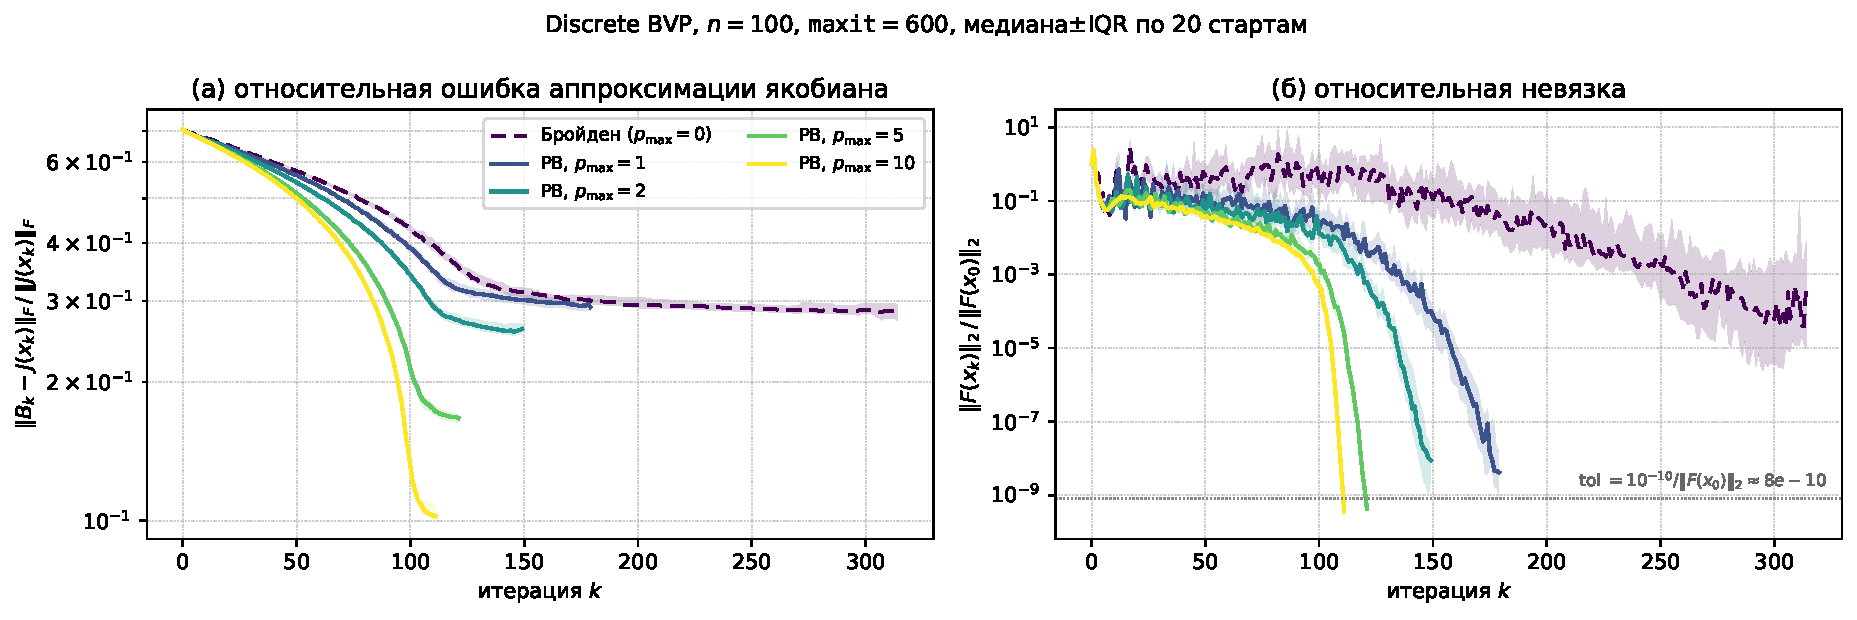
\includegraphics[width=\textwidth]{fig_sp_broyden_jacerr.pdf}
\caption{Discrete BVP, $n=100$, $20$ случайных стартов из окрестности
$x_0$ по умолчанию. Медианная траектория $\|B_k - J(x_k)\|_F$ для
классического Бройдена ($p=0$) и Projected Broyden ($p\le 5$, $p\le 10$);
затенённая полоса~--- IQR между $25$- и $75$-перцентилями. Якобиан
$J(x_k)$ вычислен аналитически.}
\label{fig:spb_jacerr}
\end{figure}

\paragraph{Корректность L-PB в высокой размерности.}
Для проверки эквивалентности рекурсии~\eqref{eq:lsp_recursion} плотной
форме~\eqref{eq:sm_update} при $m\ge p+1$ проведено сравнение на задаче
Broyden Banded (MGH~\#31, \cite{more1981}) при $n\in\{10^4, 10^5\}$ для
случайных стартов $x_0 = -0{,}1\cdot \mathbf{1} + 0{,}05\,u_i$ с
единичными $u_i\in\RR^n$ (фиксированный seed). При $n=10^4$ плотный
Projected Broyden-SM ($p\le 5$) выступает baseline'ом ($n^2=10^8$ чисел с плавающей точкой
$\approx 800$~МБ оперативной памяти, $3$ старта); при $n=10^5$ плотная
форма принципиально неприменима ($n^2=10^{10}$ чисел с плавающей точкой $\approx 80$~ГБ).
L-PB запускается с $m\in\{5,10,20\}$ ($n=10^4$, $8$ стартов) и
$m\in\{10,20\}$ ($n=10^5$, $4$ старта). Все методы~--- с
backtracking-Армихо ($c_1=10^{-4}$); критерий
$\|F\|_2 \le 10^{-10}$.

\begin{figure}[htbp]
\centering
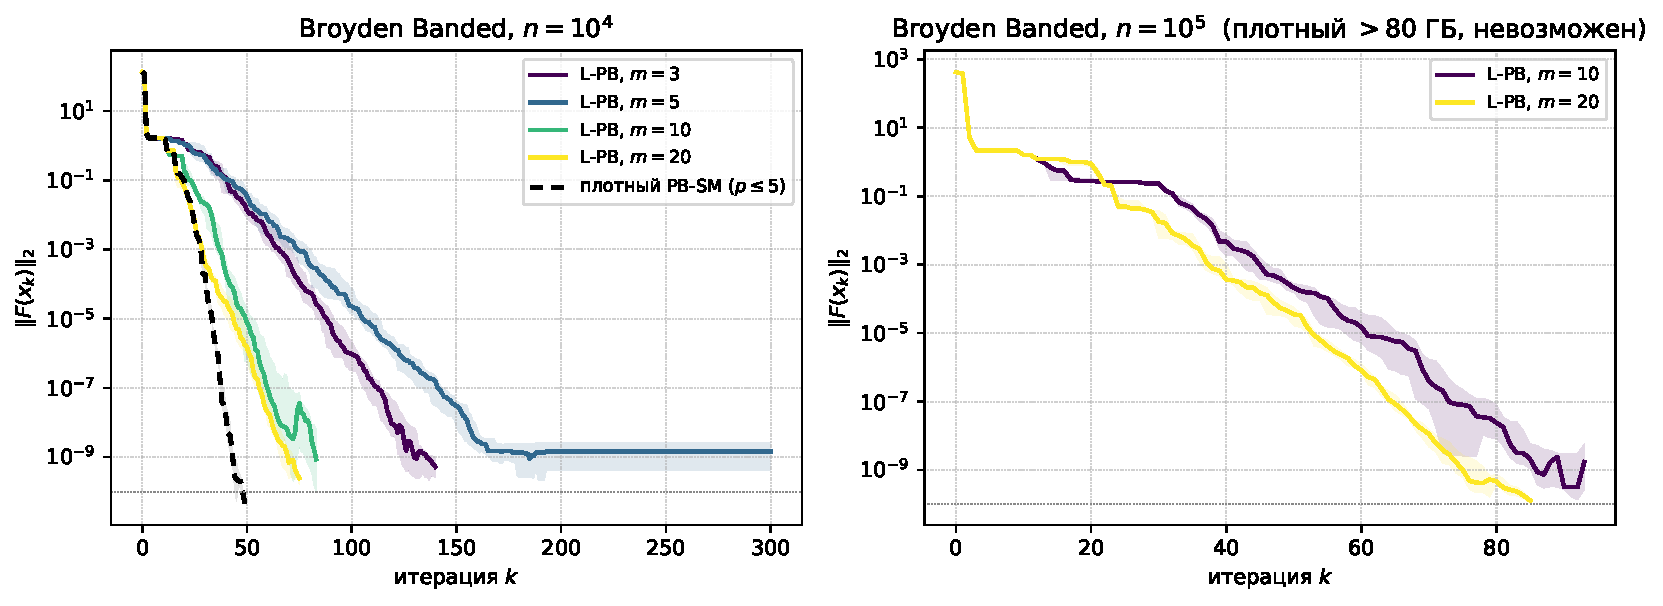
\includegraphics[width=\textwidth]{fig_highdim_conv.pdf}
\caption{Broyden Banded. Медианная траектория $\|F(x_k)\|_2$ + IQR
по случайным стартам. Слева~--- $n=10^4$ с плотным Projected Broyden-SM
($p\le 5$, чёрный пунктир) как baseline; справа~--- $n=10^5$, где
плотная форма требует $\approx 80$~ГБ оперативной памяти и
неприменима.}
\label{fig:highdim_conv}
\end{figure}

При $n=10^4$ L-PB $(m=20)$ практически точно совпадает с плотным
Projected Broyden-SM (медианы $34$ vs~$33$ итераций; кривые сливаются на
рисунке)~--- прямая эмпирическая верификация
эквивалентности~\eqref{eq:lsp_recursion} при $m\ge p+1$. Уменьшение
окна даёт пенальти: $m=10$~--- $52$ итерации, $m=5$~--- $99$ итераций
($m=5$ попадает в режим плохо обусловленного промежуточного окна, при
$m\le p+1=6$ адаптивный PB-проектор не обеспечивает запас по
$\sigma_{\min}(S_p)$). При $n=10^5$ L-PB сходится за медиану
$49$~итераций ($m=20$) и $59$~итераций ($m=10$), что качественно
согласуется с поведением при $n=10^4$~--- число итераций на сходимость
limited-memory варианта \emph{не растёт} с $n$.

\paragraph{Резюме.}
В главе введён мультисекущий Бройден с~адаптивным окном~--- ранг-$(p{+}1)$
обновление, для которого теорема~\ref{thm:bd} даёт точное разложение
Фробениус-нормы ошибки $\|E_{k+1}\|_F^2 = \|E_k\|_F^2 - \|E_k\Pi_k\|_F^2
+ \Delta_k$ и явную геометрическую константу $C_{\mathrm{PB}}$, а
следствие~\ref{cor:subspace-alignment}~--- безусловный $O(\rho_k)$-контроль
ошибки на всём подпространстве $\mathrm{col}\,S_p$. В режиме
$\mathtt{accumulate}=\text{true}$ обновление специализируется к ранг-1
форме~\eqref{eq:rank1_specialization}, что~через
Шермана--Моррисона~\eqref{eq:sm_update} ведёт к limited-memory варианту
L-PB с памятью и временем $O(nm)$ и $O(nm^2)$ соответственно. Численные
эксперименты на Discrete BVP и~Broyden Banded подтверждают
ограниченность $\|E_k\|_F$ вдоль траектории и эквивалентность L-PB
плотной форме при $m\ge p+1$, при этом число итераций на сходимость
не растёт с~$n$ вплоть до $n=10^5$.


